% LAB 3: Functions
%
% CSE/IT 107: Introduction to Programming
% New Mexico Tech
%
% Prepared by Russell White and Christopher Koch
% Spring 2015

% - Functions
%   - Positional and Optional Arguments
%   - Recursion
% - Modules
%   - import statements
%   - main() boilerplate
% - Comments and PEP-8 style
% - Keywords: def
\documentclass[11pt]{cselabheader}
\fancyhead[R]{Lab 3: Functions}
\title{Lab 3: Functions}

\begin{document}

\pagenumbering{roman}

\maketitle

\begin{figure}[H]
  \centering
  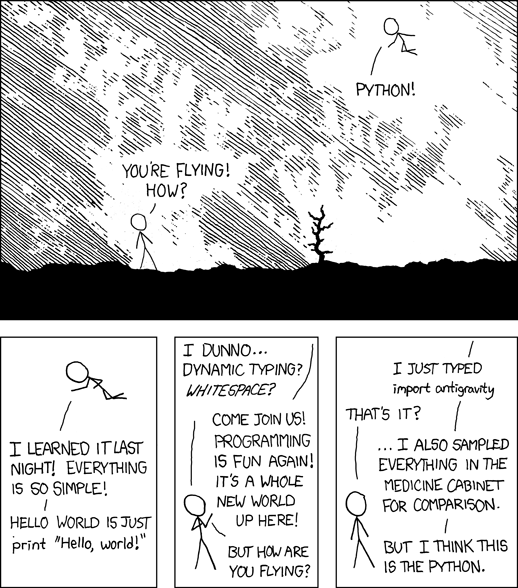
\includegraphics[width=0.85\textwidth]{img/xkcd_python.png}
  \caption{xkcd 353: Python (Source: \url{http://xkcd.com/353})}
\end{figure}

\pagebreak
\hrule
%\vspace{0.5em}
%\begin{minipage}{0.32\textwidth}

\begin{quotation}
``If you don't think carefully, you might believe that programming is just
typing statements in a programming language.''
\end{quotation}
\begin{flushright}
  --- W. Cunningham
\end{flushright}

%\vspace{2em}

\begin{quotation}
``Only ugly languages become popular. Python is the exception.''
\end{quotation}
\begin{flushright}
  --- Donald Knuth
\end{flushright}

%\vspace{2em}

\begin{quotation}
``The time you enjoy wasting is not wasted time.''
\end{quotation}
\begin{flushright}
  --- Bertrand Russell
\end{flushright}

%\end{minipage} 
%\begin{minipage}{0.68\textwidth}
%  \begin{flushright}
%  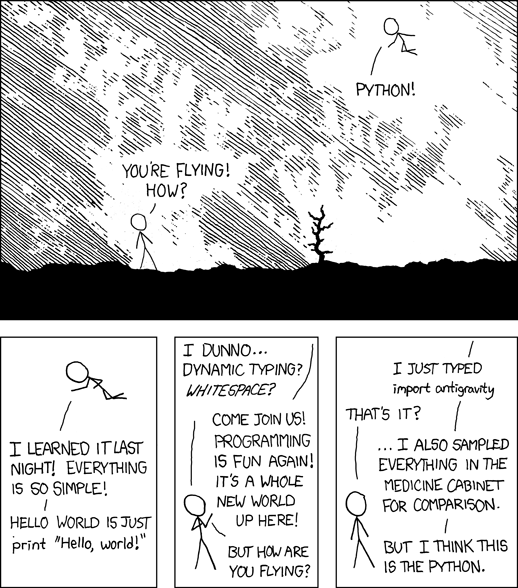
\includegraphics[width=0.97\textwidth]{img/xkcd_python.png}
%  \end{flushright}
%\end{minipage}
%\vspace{0.5em}
\hrule

\tableofcontents

\pagebreak
\pagenumbering{arabic}

\section{Introduction}
\label{sec:intro}

In the previous lab, we showed you simple control flow and how to repeat a piece
of code using \pythoninline{while}. In this lab, we will be learning how to
break a lot of code into smaller, reusable pieces called \emph{functions}.

\section{Making Calculations Shorter}
\label{sec:calc}

+=, -=, /=, etc operators

\pagebreak
\section{Functions}
\label{sec:funcs}

basic functions, def

\subsection{Summary}
\label{subsec:funcs.sum}

\subsection{Exercises}
\label{subsec:funcs.ex}

\pagebreak
\section{Conventions}
\label{sec:pep8}

In order to make code more readable, we will start requiring you to comment your
code and follow a style guide. Style guides are often used to make code easy to
read, especially if multiple people are working on a project together. If left
to their own devices, most people start conforming to their own style guide
anyway just by preferring a certain way to write something over another. For
example, common parameter of style guides is the use of a certain number of
spaces for indentation. Also, some people put spaces before each colon, and some
people do not.

\subsection{Style Guide}

We will be using PEP 8 (Python Enhancement Proposal 8 -- Style Guide for Python
Code) found at
\begin{center}
  \url{https://www.python.org/dev/peps/pep-0008/}
\end{center}

Some of the highlights:
\begin{itemize}
  \item 4 space indentation
  \item Function names should be all-lowercase with words separated by underscores.
  \item File/module/package names should have short, all-lowercase names.
  \item Comment your code with useful information. For example,

    \begin{python3code}
x = x + 1 # Increment x
    \end{python3code}

    should be avoided. It is obvious that \pythoninline{x} is being incremented.
    Instead, if you think a comment will improve code comprehension, the
    following can be useful:

    \begin{python3code}
x = x + 1 # Compensate for border
    \end{python3code}

  \item Avoid whitespace where it does not help code legibility. Never put a
    space between a function name and the parentheses when calling a function.

    \begin{python3code}
if x == 4: # do this
    print(x, y)

if x == 4 : # don't do this
    print ( x , y )
    \end{python3code}
\end{itemize}

\pagebreak
\subsection{Commenting Functions}

For commenting on functions, we will be using PEP 257 (Docstring Conventions)
found at
\begin{center}
  \url{https://www.python.org/dev/peps/pep-0257/}
\end{center}

You will be required to put a \emph{docstring} at the beginning of every
function that you code from now on. A docstring is a comment immediately
following the function definition enclosed by triple-double-quotes (\texttt{"""}).

The highlights:
\begin{itemize}
  \item For short functions, do this:

    \begin{python3code}
def midpoint(a, b):
    """Find and return the midpoint of the given a and b."""
    return (a+b)/2
    \end{python3code}

  \item For larger functions or for a longer explanation, follow this style:

    \begin{python3code}
def calculate_weekly_pay(pay_rate, hours, tax_rate):
    """Calculate the net pay after taxes given the number of hours worked 
    in a week, a pay rate, and a flat tax rate.

    Arguments:
    pay_rate -- rate of pay
    hours -- number of hours worked in one week
    tax_rate -- flat tax rate (for example, 0.15 for 15%)
    """
    pay_before_taxes = hours * pay_rate

    # Add overtime payment if necessary
    if hours > 40:
        pay_before_taxes += (hours - 40) * pay_rate * 0.5

    pay_after_taxes = pay_before_taxes * (1 - tax_rate)
    return pay_after_taxes
    \end{python3code}

\end{itemize}

\pagebreak
\section{Modules}
\label{sec:modules}

import, boilerplate

\subsection{Summary}
\label{subsec:modules.sum}

\subsection{Exercises}
\label{subsec:modules.ex}

\pagebreak
\section{Advanced Functions}
\label{sec:adv}

\subsection{Positional and Optional Arguments}
\label{subsec:adv.args}

\subsection{Recursion}
\label{subsec:adv.recursion}

\subsection{Summary}
\label{subsec:adv.sum}

\subsection{Exercises}
\label{subsec:adv.ex}

\pagebreak
\section{Submitting}

Files to submit:
\begin{itemize}
  \item 
\end{itemize}

You should submit your code as a tarball. It should contain all files
used in the exercises for this lab. The submitted file should be named
\begin{center}
  \texttt{cse107\_firstname\_lastname\_lab3.tar.gz}
\end{center}

\begin{center}
  \textbf{Upload your tarball to Canvas before the deadline.}
\end{center}


\end{document}
